\documentclass[letterpaper]{article}
\usepackage[utf8]{inputenc}
\usepackage[T1]{fontenc}
\usepackage{natbib,alifeconf}  %% The order is important

\usepackage{graphicx}
\usepackage{hyperref}
\usepackage{amsmath}


% *****************
%  Requirements:
% *****************
%
% - All pages sized consistently at 8.5 x 11 inches (US letter size).
% - PDF length <= 8 pages for full papers, <=2 pages for extended
%    abstracts (not including citations).
% - Abstract length <= 250 words.
% - No visible crop marks.
% - Images at no greater than 300 dpi, scaled at 100%.
% - Embedded open type fonts only.
% - All layers flattened.
% - No attachments.
% - All desired links active in the files.

% Note that the PDF file must not exceed 5 MB if it is to be indexed
% by Google Scholar. Additional information about Google Scholar
% can be found here:
% http://www.google.com/intl/en/scholar/inclusion.html.


% If your system does not generate letter format documents by default,
% you can use the following workflow:
% latex example
% bibtex example
% latex example ; latex example
% dvips -o example.ps -t letterSize example.dvi
% ps2pdf example.ps example.pdf


% For pdflatex users:
% The alifeconf style file loads the "graphicx" package, and
% this may lead some users of pdflatex to experience problems.
% These can be fixed by editing the alifeconf.sty file to specify:
% \usepackage[pdftex]{graphicx}
%   instead of
% \usepackage{graphicx}.
% The PDF output generated by pdflatex should match the required
% specifications and obviously the dvips and ps2pdf steps become
% unnecessary.


% Note:  Some laser printers have a serious problem printing TeX
% output. The use of ps type I fonts should avoid this problem.


\title{The challenges of cooperation for a swarm of heterogeneous robots}
\author{Paul Ecoffet$^1$, Jean-Baptiste André$^2$, Nicolas Bredeche$^1$ \\
\mbox{}\\
$^1$Institut des Systèmes Intelligents et Robotique, Sorbonne Université, Paris \\
$^2$Institut Jean-Nicod, École Normale Supérieure, Paris \\
\href{mailto:ecoffet@sorbonne-universite.fr}{ecoffet@sorbonne-universite.fr}} % email of corresponding author

% For several authors from the same institution use the same number to
% refer to one address.
%
% If the names do not fit well on one line use
%         Author 1, Author 2 ... \\ {\Large\bf Author n} ...\\ ...
%
% If the title and author information do not fit in the area
% allocated, place \setlength\titlebox{<new height>} after the
% \documentclass line where <new height> is 2.25in



\begin{document}
\maketitle

\begin{abstract}
% Abstract length should not exceed 250 words
  
\end{abstract}

\section{Introduction}

- Cooperation avec clonal Floreano
- Cooperation swarm partner choice (no evo) \cite{Aktipis2011}


In collective robotics, the accomplishment of a task for a population is often not aligned with the individual objective of each robot. Thus, a population of robots maximizing their individual gains may interfere with the execution of the collective task. How can we then align the individual goals of the agents to this collective success? This problem has been extensively studied in game theory and evolutionary biology \citep{Axelrod1981}. Several mechanisms have been identified that allow this alignment to take place \citep{West2007a}. Among these mechanisms, partner choice is an efficient mechanism. Each individual seeks to maximize his own gain and must interact with another partner. If individuals have the ability to select their partner, then it is in their interest to find the best possible partner as quickly as possible. Thus, individuals, in order to be chosen as a partner, have an interest in being more cooperative than the individually optimal action is. There is pressure to be cooperative in order to be chosen as a partner. Theoretical results have shown that for partner selection to be effective, the time spent searching for a partner compared to the time spent interacting with partners should be as short as possible \citep{Debove2015b}. Let $\beta$ be the meeting probability per time step for an individual, and $\tau$ be the cessation probability per time step of two partners after an interaction, so $\beta / \tau$ must be large for partner selection to be effective. Our goal is to identify robotic environments where partner choice is effective. To do so, we have built a pseudo-realistic environment where robots meet on patches and can interact together. We modulate our environment according to different parameters and study the emergence of partner choice behavior and the appearance of cooperation behavior under these different conditions. We have shown that for partner choice to be possible, constraints are very strong. The robot population must be very dense in order to have a very high $\beta$ encounter probability. Moreover, the interactions between two robots must be very long (very low $\tau$) in order for the search time to be small enough compared to the interaction time.

\section{Methods}

\subsection{Environment}

We define a collective forage task where $N$ robots move and consume resources in pairs in a circular arena. The resources are spread randomly throughout the arena (see Fig.~\ref{fig:env}). Resources can be seen by robots and are surrounded by patches. Robots must move on the patches to consume the resource and increase their scores. A robot alone cannot exploit a resource. When two robots are on the same patch, they can collaborate to exploit a resource. Each robot receives a payoff based on its own investment and that of its partner. Depending on its investment, a robot can act either by cheating (it invests to maximize its own gain) or by cooperating (it invests to maximize the gain of the pair). 

\begin{figure}
    \begin{center}
        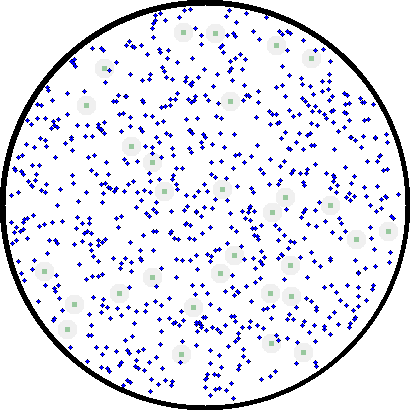
\includegraphics[width=2.5in]{media/wander_env.png}
        \vskip 0.25cm
        \caption{The environment. Each blue dot is a robot. Each green dot is a resource and the light green circle around it is the patch. Robots can see the resources, and when two robots walk on a patch, they can interact together.
        }
    \label{fig:env}
    \end{center}
\end{figure}

When two robots are on the same patch, they can choose to interact together and exploit the resource. First, each robot accesses the action that its partner intends to do, then it decides whether or not to accept the interaction. If one of the robots choose not to interact, then the resource disappears and the robots continue their course. If both robots accept, the resource disappears and they play the announced investments to get their payoffs. The robots switch then to a wandering behaviour for a certain period of time. It represents the amount of time the robots interact with each other, or a digestion period. Each robot has a probability $\tau$ of returning to the game at each iteration. The expected duration of an interaction for an agent is therefore $1/\tau$. Two robots that have interacted together may not come back to partner seeking behaviour at the same iteration. When a resource disappears, a new resource appears in the arena at the next iteration.

\subsection{Cooperation Market} \label{sec:market}
According to the theoretical results on partner choice \citep{Debove2015b}, the efficiency of this strategy depends on the meeting probability of an agent ($\beta$) and the split probability of an interaction ($\tau$). If the meeting probability is big compared to the split probability, that is $\beta/\tau$ is large, then partner choice is a viable strategy and can emerge. Indeed, for partner choice to be effective, when an agent refuses to interact with a partner, it must do so because its expectation of gain in finding a better partner outweighs the gain missed by rejecting the interaction with the wrong partner and the implied cost paid by looking for a new partner. Thus, if search time is short compared to interaction time, it is profitable to spend more time searching for a good partner than interacting with more uncooperative partners.

The $\beta$ parameter is determined by the ability of the robots to meet on a patch and varies as the robots evolve, but also depending on the density of robots in the arena, and especially the robots that are also seeking for partner. In our model, the split probability $\tau$ parameter is chosen experimentally.

\subsection{Objective function}

When two robots interact with each other, they earn a gain determined by the investment of the two agents. The gain of an agent $a_i$ investing $x_i$ with its partner $a_j$ investing $x_j$ is determined by the function $P(x_i, x_j)$ described in the equation~\ref{eq:payoff}.

\begin{align}
PG(x_i, x_j) &= \frac{a}{2} (x_i + x_j) \\
PD(x_j) &= \frac{b}{2} (x_j) \\
C(x_i) &= \frac{1}{2} x_i^2 \\
P(x_i, x_j)& = PG(x_i, x_j) + PD(x_j) - C(x_i) \label{eq:payoff}
\end{align}

This function is a mixture of a public good ($PG$, modulated by $a$) and a prisoner's dilemma ($PD$, modulated by $b$) and a quadratic cost $C$. For $a_i$ to maximize its individual gain ($P(x_i, x_j)$), the optimal investment is $x_d = \frac{a}{2}$, which correspond to the defective behaviour. For the group to maximize their total gain, both agents must invest $\hat{x} = a + \frac{b}{2}$, which correspond to the cooperative behaviour. The Figure~\ref{fig:payoff} is a plot of the payoff function with different partner's investment values.



\begin{figure}[htpb]
    \centering
    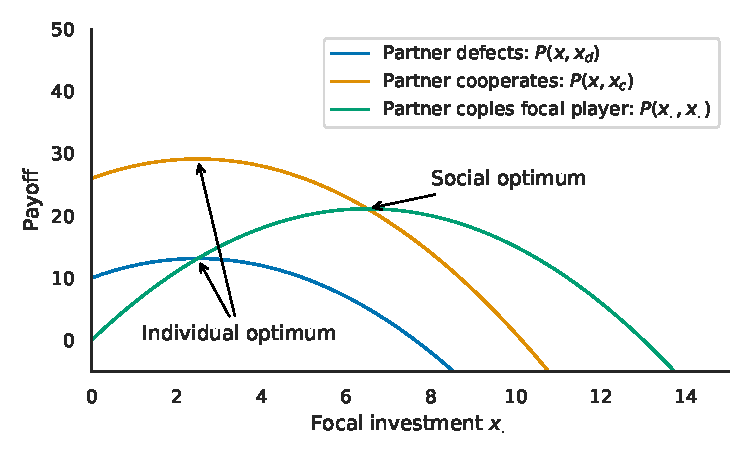
\includegraphics[width=\columnwidth]{media/payoff.pdf}
    \caption{Payoff function with different partner's investment value. The individually optimal investment is $x_d = \frac{a}{2}$ whatever the constant value the partner invests, which correspond to a defective behaviour. If both robots invest the same value, then the socially optimal investment is $\hat{x} = a + \frac{b}{2}$, which correspond to a cooperative behaviour.}
    \label{fig:payoff}
\end{figure}

\subsection{Controller}

The robot control system is composed of the investment value ($x \in [0, 10]$) during interaction and two decision modules: The movement module and the partner choice module. The robot always invests the same value and the modules remain fixed throughout the task. 

The movement module is an artificial neural network with 1 hidden layer of 10 neurons. All the nodes have a $\tanh$ activation function. The input of the network is the detailed information from the 8 sensors of the robot. The network gives as output the speed of translation and rotation between $]-1, 1[$. These values are then resized to match the maximum translation and rotation speeds of the robot.

The partner choice module is also a artificial neural network. It is activated only when an agent is with another agent on the same patch. This network receives as inputs the investment level of the robot as well as the investment level of its partner. It is composed of 1 hidden layer of 3 neurons and has a $\tanh$ activation function. It gives as output a value ($a \in ]-1, 1[$), which correspond to the response to the partner. If the output is greater than 0, then the robot accepts the interaction, otherwise it refuses it and the interaction does not take place.  The details of the inputs of each network are given in the Table~\ref{tab:ann_params}.

All neural network weights are bounded in the range $]-10, 10[$. In total, the two neural networks consist of 368 weights.

\begin{table}
    \centering
    \begin{tabular}{cc}
        \hline
        \textbf{Input} & \textbf{Value}  \\
        \hline
        \textbf{Movement module} & \\
        \textit{Per sensor ($\times 8$)}& \\
        Distance to Robot &  $]0, 1[$ if in range else 1 \\
        Distance to Wall & $]0, 1[$ if in range else 1  \\
        Distance to Resource & $]0, 1[$ if in range else 1  \\
        Robot on the patch & 0 or 1 \\
        \hline
        \textbf{Partner choice module} & \\
        Partner's investment & $]0, 10[$ \\
        Robot's own investment & $]0, 10[$ \\
        \hline
    \end{tabular}
    \caption{Neural Networks inputs}
    \label{tab:ann_params}
\end{table}

\subsection{Phenotypic variability} \label{sec:phenovar}

\citet{McNamara2010c} reviews different works that have shown the importance of variability in the level of investment in the population to allow agents' selectivity and thus enable the appearance of partner choice. Indeed, for selectivity to be a useful skill, the variability of investments between agents must be big enough so that the payoff variation between two different partners is sufficiently beneficial. In this case, selective robots have the upper hand against undiscriminating robots.

This variability can be present by itself or enforced either with a very high mutation strength for the gene encoding the investment level for each agent, or by adding a noise to the genetically encoded investment level for each agent that will remain the same throughout the task. 

\subsection{Learning}

The weights of the neural networks and the investment value of a robot constitute its genome. In total, a robot has $369$ genes, the $g_x$ gene to encode the investment level and the 368 $g_{w_i}\,\forall i \in 0..368$ genes to encode the weights of the two neural networks. The value of $g_x$ is in $]0, 1[$, the investment level $x$ of the robot is defined by $x = 10 \times g_x$. The values of $g_{w_i}$ are in $]-10, 10[$.

At the beginning of learning, the $g_{w_i}$ genes are randomly initialized in the range $]-1, 1[$ and the $g_x$ gene is randomly initialized in $]0, 1[$.

We use the fitness-proportionate evolutionary algorithm described below for the learning of our robots. After each generation, the total payoffs of the agents represent their fitnesses. Thus, the fitness $F_i$ of the robot $i$  which had accepted $n$ interactions is described by (Eq.~\ref{eq:totalpayoff})


\begin{equation}
    F_i = \frac{1}{\tau} \sum_{j=0}^{n} P(x_i, x_j) \label{eq:totalpayoff}
\end{equation}  

with $x_j$ being the investment value of the robot's partner at the $j^{th}$ interaction. Each payoff is weighted by $\tau$ to normalize the total payoff gains by robots between conditions where $\tau$ varies.

A new generation of robots is generated by randomly drawing the agents' genomes in proportion to their fitnesses. Then a mutation operation is applied to each agent of the new generation. Each $g_i$ gene of a robot has a probability $\mu = 0.01$ to mutate. If the gene is selected, then it has a probability of $0.1$ to mutate according to a uniform distribution $\mathcal{U}(]-10, 10[)$ and a probability of $0.9$ to mutate according to a normal distribution $\mathcal{N}(g_i, \sigma)$ with $\sigma = \sigma_w = 0.1$ for the weight genes and $\sigma = \sigma_x = 0.1$ for the investment gene. The new generation then performs the task and the process is repeated for $G = 200$ generations (see Table~\ref{tab:env_params} for a list of all the parameters). 

\begin{table}
    \centering
    \begin{tabular}{clc}
        \hline
        \textbf{Param} & \textbf{Description}  & \textbf{Value} \\
        \hline
        \multicolumn{3}{l}{\textbf{Payoff}} \\
        $a$ & Public good weight & 5 \\
        $b$ & Prisoner's dilemma weight & 3 \\
        %\hline
        \multicolumn{3}{l}{\textbf{Environment}} \\
        $T$ & Number of iterations per generation & $100\,000$ \\
        $G$ & Number of generations per run & $200$ \\
        & Arena diameter & 400px \\
        & Robot size & 4px \\
        & Robot max speed & 2px/iteration \\
        $\omega$ & Number of patches & 30 \\
        $\tau$ & End of interaction probability & \\
        %\hline
        \multicolumn{3}{l}{\textbf{Evolution hyper-parameters}} \\
        $\mu$ & mutation probability & 0.01 \\
        $\sigma_w$ & mutation strength of weight genes & 0.1 \\
        $\sigma_x$ & mutation strength of investment gene& 0.1 \\
        \hline
    \end{tabular}
    \caption{Experiment parameters}
    \label{tab:env_params}
\end{table}

\section{Results}

\subsection{Experimental setup}

The environment is a circular arena with a diameter of 400px. The robots are 4px diameter disks. The robots have 8 equally distributed sensors with a range of 96px giving them information about their surroundings, such as the presence of other robots, of a resource or of a wall. The robots move through the environment at a maximum translation speed of 2px/iteration and a rotational speed of $30^\circ$/iteration. $N$ robots are spread randomly in the environment and 30 resources are randomly scattered throughout the arena. Each generation lasts $T = 100\,000$ iterations. The environment is represented in Figure~\ref{fig:env}.

The results presented below are obtained by the behavioral study of the $200^{th}$ generation.  We ran 24 simulations per condition in all experiments.

We have studied the influence of several factors that may facilitate the emergence of partner choice and cooperation behaviours: (i) the effect of population size (ii) the effect of the duration of interactions by changing the split probability ($\tau$), and (iii) the strength of the investment gene mutation ($\sigma_x$). 

\subsection{Effect of the population size}

We first wanted to test the impact of the population size on the emergence of partner choice. Does a bigger population size positively impact the emergence of cooperative behavior? %question
To test the emergence of the cooperation behavior by partner choice, we set the parameters to be the most favourable for its emergence. We set $\tau = 0$ and the evaluation duration $T = 100\,000$ in order to grant a long search time for the robots and a very engaging commitment if they accept the interaction. %expe
At $N = 50$, robots plays the defective strategy. the average investment level is very close to the social optimum for $N = 1\,000$ (see Figure~\ref{fig:do_coop}). % results 
The robots evolve a cooperative behavior for $N$ sufficiently large. The denser the population, the higher the probability of encounters $\beta$ is. Thus, with 50 robots in the arena, the robots are unable to meet and sample enough partners to be selective before the end of the generation. Moreover, the robots are racing to find a partner quickly. Indeed, with $\tau = 0$, the more the task advances in time, the fewer agents are available in the arena and thus the more $\beta$ decreases throughout the evaluation. % interpretation



\begin{figure}[tbhp]
    \begin{center}
        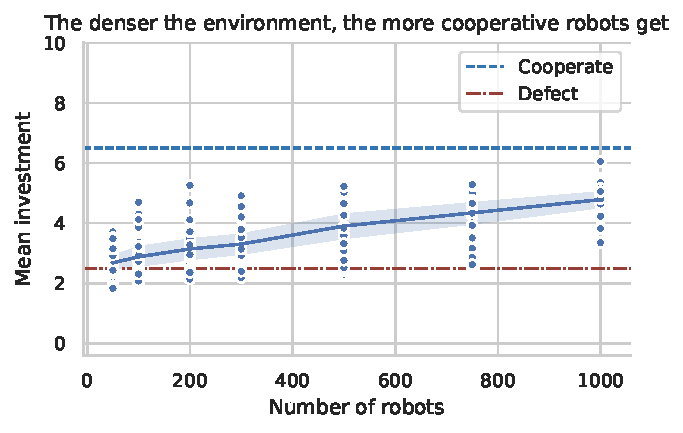
\includegraphics[width=3in]{media/wander_do_coop.pdf}
        \vskip 0.25cm
        \caption{The larger the population, the higher the agents' level of investment.
        Mean investment of the population for 24 simulations per condition with a split probability $\tau = 0$ and a mutation strength for investment $\sigma_x = 0.1$. When the population is large, agents can easily find a partner and can be more selective. The pressure to invest a lot is then greater due to the effect of the partner choice.
        }
        \label{fig:do_coop}
    \end{center}
\end{figure}


To show the importance of partner choice in the evolution of this cooperative behavior, %question
we built a control condition where we deactivate the agents' ability to know their partner's investment in order to accept or not accept an interaction. % expe
In this condition, whatever the number of agents in the environment, the average investment level is always $x_d$, that is a defective behaviour (see Fig.~\ref{fig:control}). % results
In this situation, agents have no way to be selective and cannot choose a cooperative robot over a non-cooperative one. Thus, cooperative robots are not preferentially selected as partners and there is no incentive to invest more than the individual optimum. There is no selection pressure in favor of the most cooperative agents. % interpretation

\begin{figure}[tbhp]
    \begin{center}
        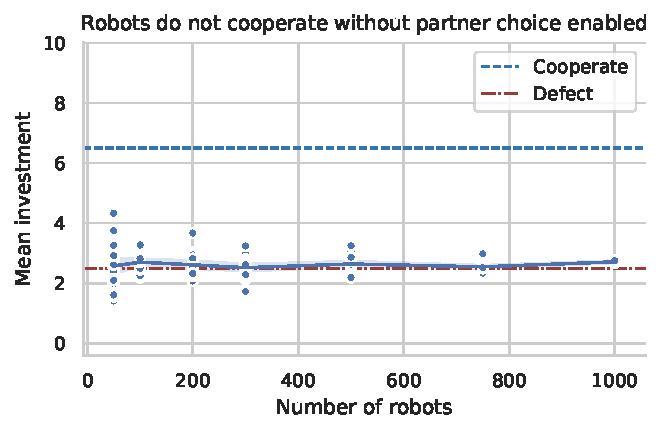
\includegraphics[width=3in]{media/wander_control.pdf}
        \vskip 0.25cm
        \caption{Robots never cooperate in control condition. Mean investment of the population for 24 simulations per condition with a split probability $\tau = 0$ and a mutation strength of investment $\sigma_x = 0.1$. Robots never cooperate whatever the number of robots $N$ in the environment. Without access to their potential partner's investment level, agents cannot be selective and partner selection is impossible. Agents are under no pressure to invest a lot to be chosen. Therefore, they all play at the individually optimal investment level.
        }
        \label{fig:control}
    \end{center}
\end{figure}


\subsection{Effect of the interaction length}

%question
%expe
%results
%interpretation

According to the theoretical results, the longer the interaction, the greater the influence of the choice of partner (see section~\nameref{sec:market}). We test the reality of this prediction in our experimental setup. % question
To do this, we vary the split probability $\tau$.  % expe
The larger $\tau$ is, the shorter the interaction. When the split probability $\tau$ is null or low and the population size $N$ is large, the robots invest in a collectively optimal way and have a cooperative behavior (see Fig.~\ref{fig:corr_tau_comp}. % results
The larger the $\tau$ becomes, the less cooperative the robots are even for a high population size. The robots plays systematically a defective investment with $\tau \geq 1\times 10^{-3}$ Thus, increasing the duration of interactions has a positive effect on the appearance of cooperative behavior by partner choice. % interpretation


\begin{figure}[tbhp]
    \begin{center}
        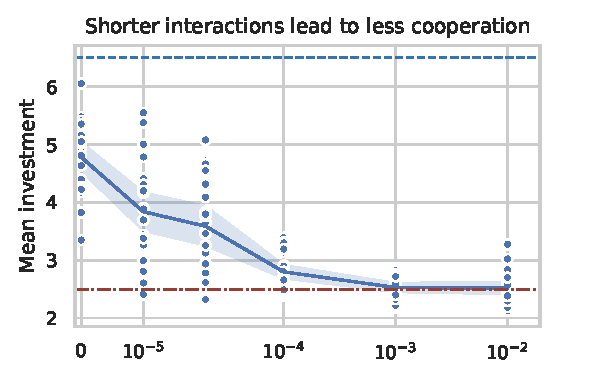
\includegraphics[width=3.3in]{media/wander_corr_tau_coop_pop1000.pdf}
        \vskip 0.25cm
        \caption{The smaller the split probability $\tau$ is, the more cooperative robots get. The robots invest cooperatively for $\tau \leq 2\times 10 ^{-5}$, and have a defective behaviour for $\tau > 2 \times 10^{-5}$. The higher $\tau$ is, the less long are the interaction and the more profitable it is to interact with a lot of bad partner compared to looking for a good partner and interact with it.
        }
        \label{fig:corr_tau_comp}
    \end{center}
\end{figure}


\subsection{Effect of the mutation strength}

As explained in the section \nameref{sec:phenovar}, different works have shown the importance of variability in the level of investment in the population to allow agents' selectivity and thus enable the appearance of partner choice \citep{McNamara2010c}.
We test the influence of higher phenotypic variability in our task. % Question
To do so, we (i) modified the strength $\sigma_x$ of the Gaussian mutation on the gene encoding the robot investment level and (ii) applied a constant noise on the robot investment level during a generation. % expe
We observe very minor differences in the average investment level between the different simulations (see Fig~\ref{fig:varmut}). However, we note the presence of less variability between simulations when the mutation level is high. This can be explained by a more rapid convergence towards the optimal investment level. % resultats
The fact that the variability of investment in the environment plays very little role in our task may be explained by the fact that all possible levels of investment are present in the first generation. The ability to be selective in the choice of partner may therefore emerge before the population is completely homogeneous and thus selectivity becomes an unnecessary skill. % interpretation


\begin{figure}[tbhp]
    \begin{center}
        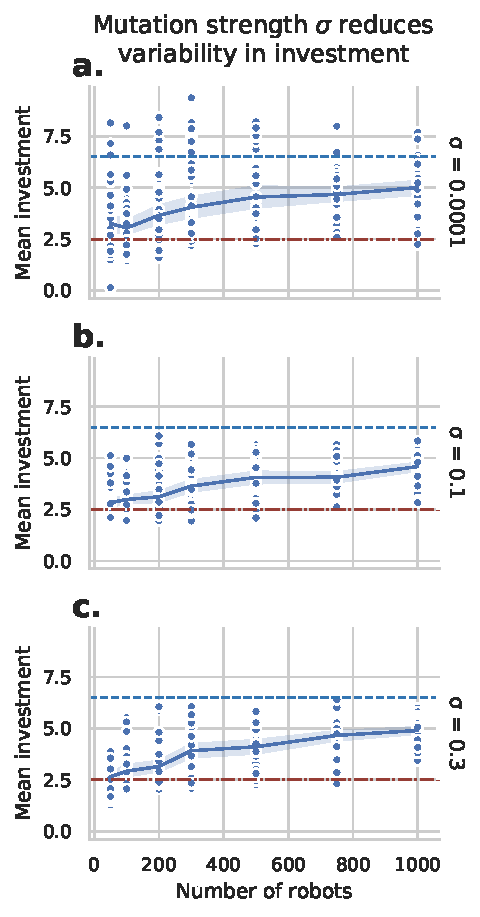
\includegraphics[width=2.4in]{media/wander_varmut.pdf}
        \vskip 0.25cm
        \caption{A higher mutation strength has no impact on average cooperation but reduces variance in investment between simulations.
        Average investment in the population for 24 simulations per condition with $\tau = 0$. The addition of phenotypic variability facilitates the appearance of agent selectivity at low investment mutation strength \citep{McNamara2010c}. Here, variations in mutation strength for investment $\sigma_x$ %or the addition of phenotypic variability
        have only a small impact on the final investment level of the agents. This may be due to the fact that all possible investment levels are represented at the Initialization of the simulation.
        }
    \label{fig:varmut}
    \end{center}
\end{figure}



\subsection{Control: population size vs number of generations}

The difference in population size between low (50 robots) and high (1000 robots) population conditions could be explained by the lower number of evaluations that the 50 robot conditions have to evolve cooperative behaviour. Indeed, with the number of generations being constant ($G = 200$), the number of evaluations for the condition with 50 robots is $50 \times 200 = $10,000 and for the conditions with 1000 robots is $1,000 \times 200 = 200,000$. This difference in the number of evaluations could explain why cooperative behaviour has evolved in the conditions where $N$ is large and not in those where $N$ is small. Has the evolution converged in the small $N$ conditions? % Question
To test the impact of this number of evaluations, we run a new control condition of 24 simulations with $G = 4,000$ for a population of $N=50$ robots, offering $200\,000$ evaluations. % Method
The difference between the condition $N=50, G=200$ and $N=50, G=4000$ is marginal, but the difference between these conditions at the condition $N=1\,000, G=200$ is very large (Fig.~\ref{fig:gencomp}). Adding more generations does not improve the level of cooperation achieved for conditions with a small population. % results
It is therefore the too low encounter probability $\beta$ that blocks the emergence of cooperative behavior under these conditions, not the fewer evaluations. % interpretation


\begin{figure}[tbhp]
    \begin{center}
        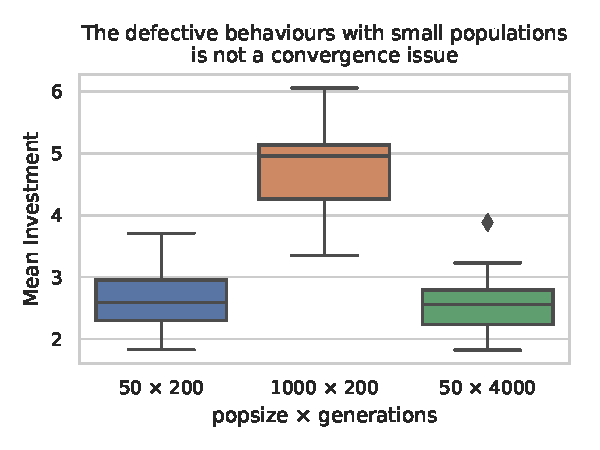
\includegraphics[width=3.3in]{media/wander_comp_genpop.pdf}
        \vskip 0.25cm
        \caption{More generations with small population does not lead to cooperative behaviour. The differences in robot investment between conditions $N=50$ and $N=1000$ cannot be attributed to fewer evaluations for small populations.
        }
        \label{fig:gencomp}
    \end{center}
\end{figure}


\subsection{Control: Wandering vs Teleportation}


Finally, we do a final control to test the influence of the wandering behaviour. Does this facilitate or not the emergence of cooperation by partner choice? % Question
To test this, we compare the task with digestion time by wandering with a task with digestion time outside the arena. In this second condition, after one robot has interacted with another, it is placed outside the arena and has a $\tau$ probability of returning to the arena at each time step. When a robot is placed back into the arena, it is randomly placed back into the arena. This second condition is closer to the numerical simulations present in \citet{Debove2015c} than the wandering condition. We compare the results with the wandering condition and the condition outside the arena for several values of split probability $\tau$. % 2) Expe
We find that in the wandering condition as well as in the off-arena condition, when the probability of split is low ($\tau < 1\times 10^{-5}$), the robots invest cooperatively. We also find that in the off-arena condition, the robots remain cooperative for higher values of split probability. For even higher split probabilities, the robots no longer have cooperative behaviors whatever the condition. % results
The off-arena condition is more robust than the wander condition. Indeed, for higher split probability values, the agents still behave cooperatively. This can be explained by the fact that the arena is less crowded than in the wander condition. Indeed, a robot necessarily crosses potential partners in the off-arena condition, and is not blocked by agents in their digestion phase, as would be the case in the wander condition. Thus, the $\beta$ encounter probability is greater in the off-arena condition than in the wander condition. % 4) interpretation

\begin{figure}[tbhp]
    \begin{center}
        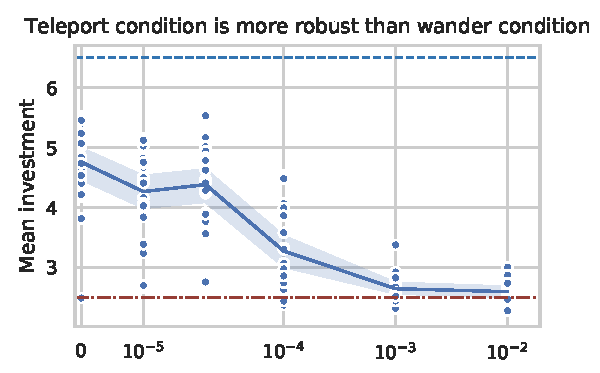
\includegraphics[width=3.3in]{media/wander_corr_tau_coop_pop1000_tp.pdf}
        \vskip 0.25cm
        \caption{Robots act cooperatively in both the wander and off-arena conditions for low split probability $\tau$. The off-arena condition is more robust to middle range values of $\tau$ than the wander condition.
        }
        \label{fig:comp_tau_wander_tp}
    \end{center}
\end{figure}



\section{Conclusion}



\section{Acknowledgements}



\footnotesize
\bibliographystyle{apalike}
\bibliography{references}

\clearpage

\section{Supplementary}

\begin{figure}[tbhp]
    \begin{center}
        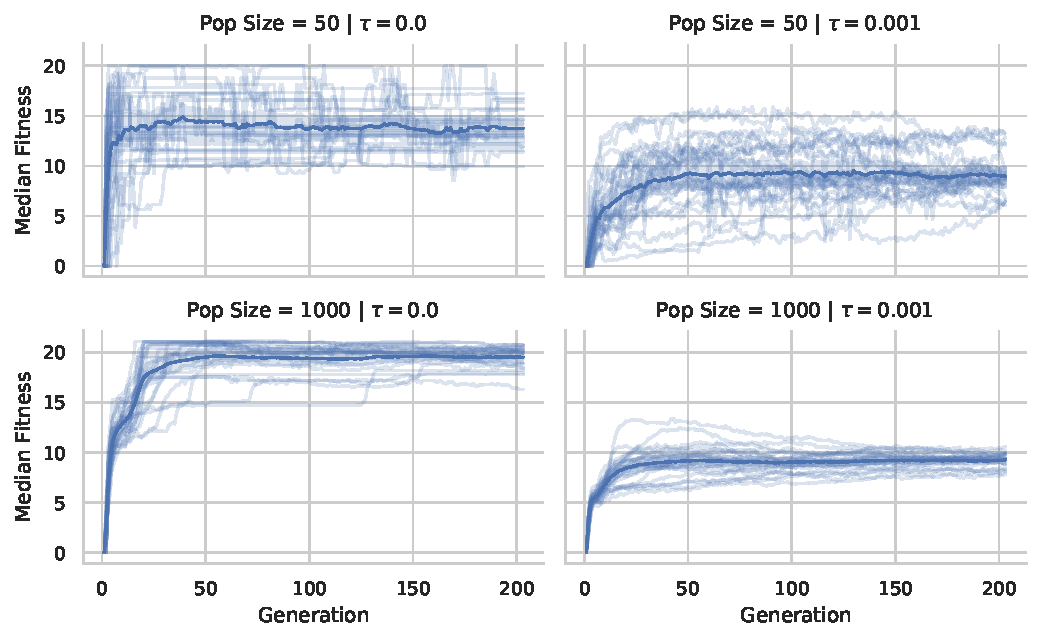
\includegraphics[width=3.3in]{media/wander_all_fit.pdf}
        \vskip 0.25cm
        \caption{Fitness is super noisy
        }
        \label{fig:allfit}
    \end{center}
\end{figure}


\begin{figure}[tbhp]
    \begin{center}
        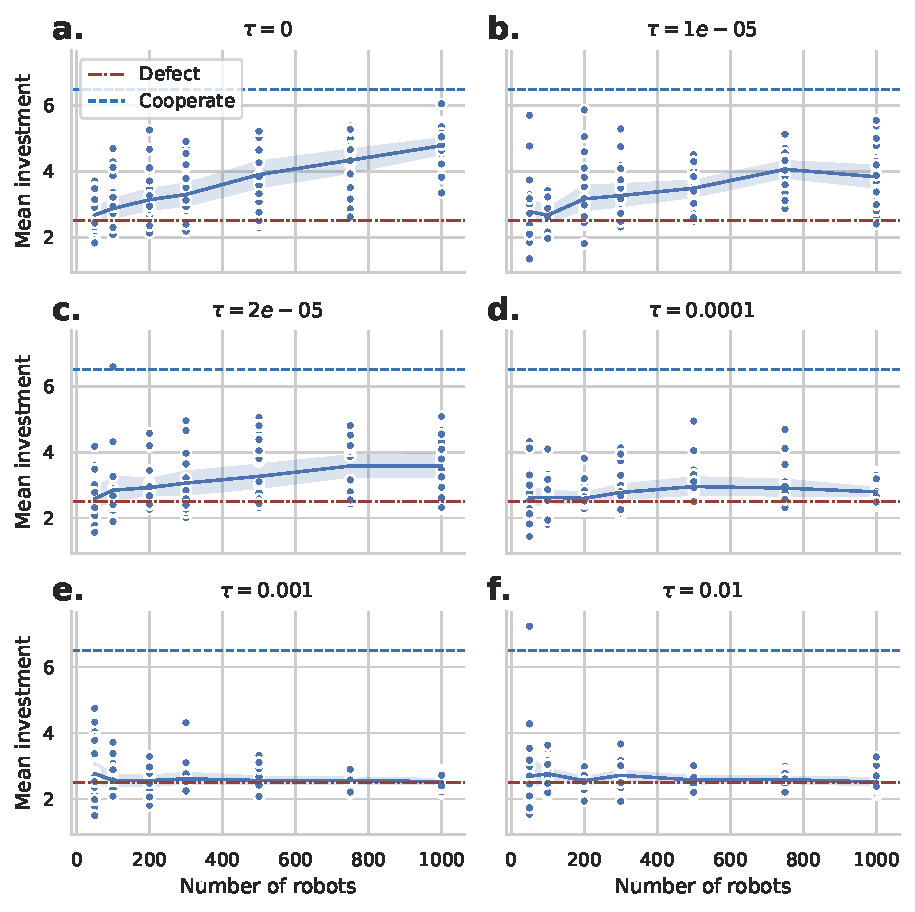
\includegraphics[width=3.3in]{media/wander_vartau.pdf}
        \vskip 0.25cm
        \caption{Average investment over 24 simulations per condition with $\sigma = 0.1$. As a function of the duration of interactions between agents ($\tau$), the average level of investment for large populations varies greatly. \textbf{a. b.} If the interactions are very long (small $\tau$), then the search time is really very small compared to the interaction time, and the search for a partner is de facto very cheap. Agents would rather spend a lot of time finding a good partner than interact with the first partner they meet. There is therefore a lot of pressure to invest a lot so as to be chosen as a partner and agents invest at the socially optimal level. \textbf{c. d.} If the interactions are very short (high $\tau$), then the search time becomes very important compared to the interaction time, and the search for a partner becomes de facto very expensive. Agents would rather have many interactions with uncooperative partners than spend a lot of time searching for an efficient partner. There is therefore no pressure to invest a lot to be chosen as a partner and agents invest at the individually optimal level.
        }
        \label{fig:vartau}
    \end{center}
\end{figure}

\begin{figure}[tbhp]
    \begin{center}
        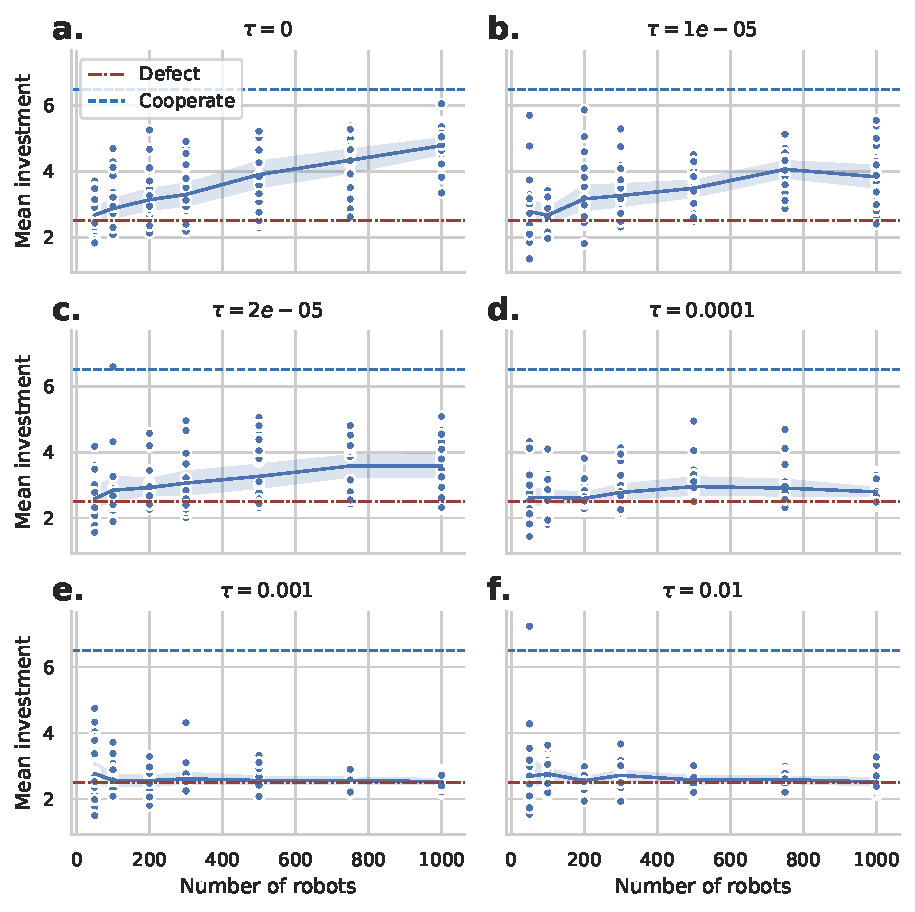
\includegraphics[width=3.3in]{media/wander_vartau.pdf}
        \vskip 0.25cm
        \caption{TP VERSION, ARENA 120px, NOT STRICTLY THE SAME
        }
        \label{fig:tp_vartau}
    \end{center}
\end{figure}


\begin{figure}[tbhp]
    \begin{center}
        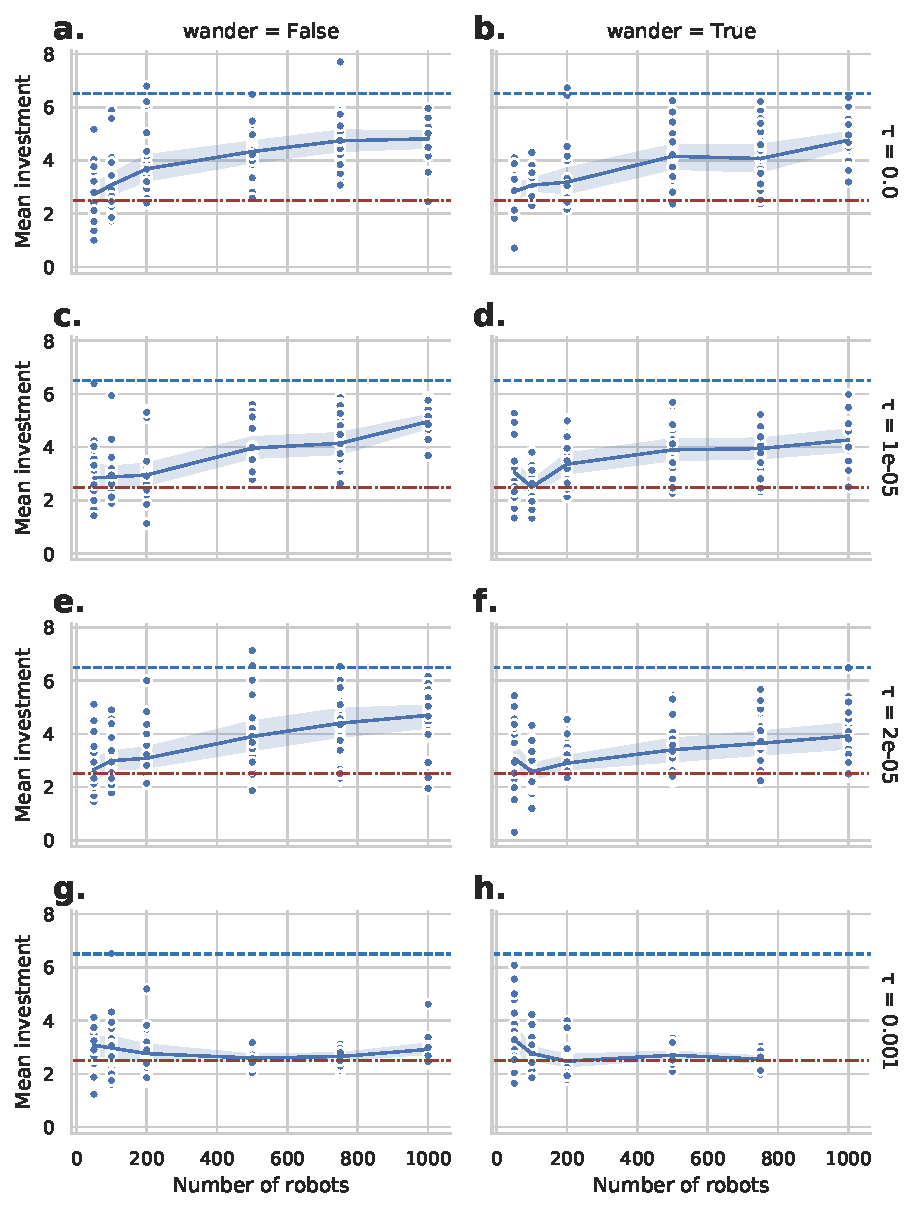
\includegraphics[width=3.3in]{media/wander.pdf}
        \vskip 0.25cm
        \caption{Average investment over 24 simulations per condition with $\sigma = 0.1$. xx TODO
        }
        \label{fig:wander}
    \end{center}
\end{figure}




\end{document}
